\newpage
Моя задача на данный семестр . \\
\begin{enumerate}
%\item сбор и анализ истории переписки мессенджеров;
\item преобразование собранной информации в читаемый вид;
\item добавление новых функций к уже имеющимся.
\end{enumerate}
Для упрощения разобьем задачу, на подзадачи
\begin{enumerate}
\item Создание веток(branch), и распределенная работа программистов. 
\item Визуализация данных
\item Выбор и описание утилит для преобразования
\item XSTL
\item Показать результат
\item Функция чтения контактной книги pidgin
\item Функция сбора используемых учётных записей pidgin
\item Описать как работает. SAP и DOM модель разбора xml
\item Функция сбора дополнительных данных skype
\end{enumerate}
\chapter*{Создание веток(branch), и распределенная работа программистов.}
Допустим мы приступаем к задаче. котороая займет больше одного дня/недели. Разработка ПО в комманде подразумевает частое создание коммитов. Это позволяет чаще получать измения и избегать кофликтов. 

Но если задача длинная, и мы будем коммитить полу сделанную задачу, то это будет как минимум мешать другим разработчикам, как максимум сделает проект неработоспособным.[2]

Однако неделать коммиты несколько дней тоже плохой вариант. Вот для этого и существуют другие ветки. Они позволяют нам вносить изменения, не мешаю и этом остальным разработчикам. Или же работать над несколькими ветками одновременно.

Ветка - это снимок репозитария в сделанный в прошлом, в который не попадают коммиты из основной ветки после момента создания.

\chapter*{Визуализация данных}
Визуализация собранной информации очень важный момент создания подобного рода комплексов, т.к. это является главной задачей нашего продукта. 

Список возможных вариантов конвертации XML
\begin{enumerate}
\item CSV
\item HTML
\item TXT
\item SQL
\end{enumerate}
Самым удобным оказался HTML.
\chapter*{Выбор и описание утилит для преобразования}
В основном XML можно записать в SQL БД и затем выводить записи БД в ввиде HTML страничек, испольюуя к примеру PHP. Однако это сложно и не к чему, мы можем воспользоваться язком преобразования XSLT. Это в разы быстрее, проще и надежней.
\chapter*{XSTL}
\\XSLT (eXtensible Stylesheet Language Transformations) — язык преобразования XML-документов. Спецификация XSLT входит в состав XSL и является рекомендацией W3C.
При применении таблицы стилей XSLT, состоящей из набора шаблонов, к XML-документу (исходное дерево) образуется конечное дерево, которое может быть сериализовано в виде XML-документа, XHTML-документа (только для XSLT 2.0), HTML-документа или простого текстового файла. Правила выбора (и, отчасти, преобразования) данных из исходного дерева пишутся на языке запросов XPath.
XSLT имеет множество различных применений, в основном в области веб-программирования и генерации отчётов. Одной из задач, решаемых языком XSLT, является отделение данных от их представления, как часть общей парадигмы MVC (англ. Model-view-controller). Другой стандартной задачей является преобразование XML-документов из одной XML-схемы в другую.
\chapter*{Показать результат}
\begin{figure}[h]
\center{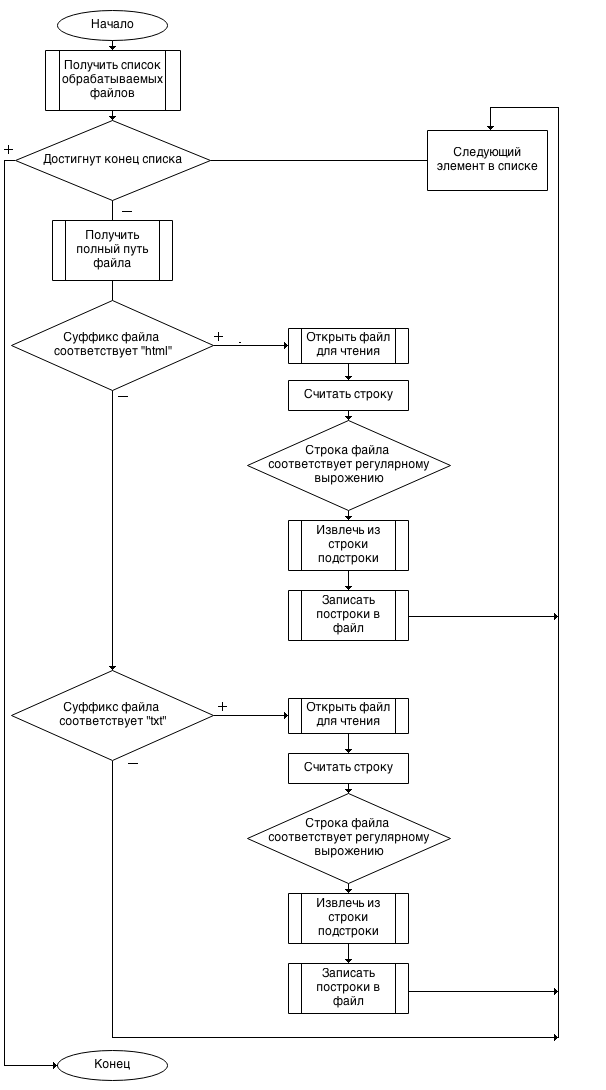
\includegraphics[width=0.5\linewidth]{Pars_pidgin_log}}
\caption{Результат преобразования XML в XSLT}
\label{pic:xml_to_xslt}
\end{figure}
\chapter*{функция чтения контактной книги pidgin}
Интересующие нас данные находятся в %путь написать тут%
\chapter*{функция сбора используемых аккаунтов pidgin}
Интересующие нас данные находятся в той же папке %путь написать тут%
\chapter*{Описать как работает SAP и DOM модель разбора xml}
[1]%Дернуть из книги%
\chapter*{функция сбора дополнительных данных skype}
Список использованной литературы:
1 -  Технология XSLT Валиков Алексей 2002г. ссылка http://www.e-reading.ws/book.php?book=1016301
2 -  GIT Pro Глава 3.1 Scott Chacon 2014г. ссылка 